While the inference servers discussed so far have exclusively utilized GPU resources, servers are easily portable and can run on other processing platforms. In particular, we have studied running the Mini-AOD workflow with servers on CPUs and Graphcore Intelligence Processing Units (IPUs)~\cite{Graphcore}.

\subsection{CPU fallback server}
\label{sec:fallback}
%As discussed in Section~\ref{sec:sonic_benefits}, SONIC can factorize the ML software frameworks out of the client. Therefore, SONIC can be used as the default approach for inference even on local CPUs, eliminating the need to integrate third-party direct ML inference framework support into the experiment software (CMSSW). In addition, w
When running with remote servers, one potentially common and important failure mode is communication errors between clients and servers. In order to support automatic local CPU inference as a backup option when communication failures occur with remote servers, the SONIC implementation includes a service that can launch a Triton server using local CPU resources for any SONIC-compatible models, referred to as a ``fallback server''. Fallback servers can also be used for inferences when third-party ML frameworks are not supported yet for direct inferences. 

Ideally, the use of fallback servers should have minimal impact on per-event throughput relative to running direct-inference jobs without SONIC. This is contingent on two factors. Firstly, the latency introduced by sending data to/from local servers must be negligible. Secondly, servers should introduce minimal overhead in order to consume as few CPU resources as possible beyond what is needed to perform inference. The first concern can be resolved using the shared-memory option, which skips the gRPC communications and directly pass between servers and clients the data in a certain memory chunk. In reality, the gRPC overhead in most cases is found to be negligible. For the second concern, since local servers are running on the same CPUs as the other modules in the workflow, scheduling should be placed to avoid CPU thread contention between the two. This implies synchronous mode is preferred for local CPU fallback servers. Inference tasks should not create extra threads to avoid contentions. In the experiments we have found that more inference threads than the CMSSW job threads will slow processings down dramatically.

After some explorations, for the local CPU inferences we decide to choose to run in synchronous mode, with the number of model instances set to the number of threads per job, and number of inference thread always 1. This way it can mimic the direct inference and avoid thread over-subscriptions as much as possible. We compare the throughputs between direct inferences and SONIC with local CPU servers with such configurations. Tests were performed using resources at the Purdue Tier-2 cluster with the CPU-only nodes. There are $n_{\text{CPU}}=20$ Intel E5-2660 CPU cores on one node, and hyperthreading is disabled to ensure more stable results. For all tests, the CPU nodes are always saturated by having the product of the number of jobs ($n_j$) and number of threads per job ($n_T$) to be the number of CPU cores: $n_j\times n_T = n_{\text{CPU}} = 20$. We scan the throughput as a function of the number of threads, as shown in Fig.~\ref{fig:throughput_cpu}. After optimizations, the throughputs of running on the local CPU fallback server are very similar to direct inference now. The higher throughputs in some cases are due to more recent versions of ONNX inference version installed inside the server, which can be controlled in the real productions.

\begin{figure}
    \centering
    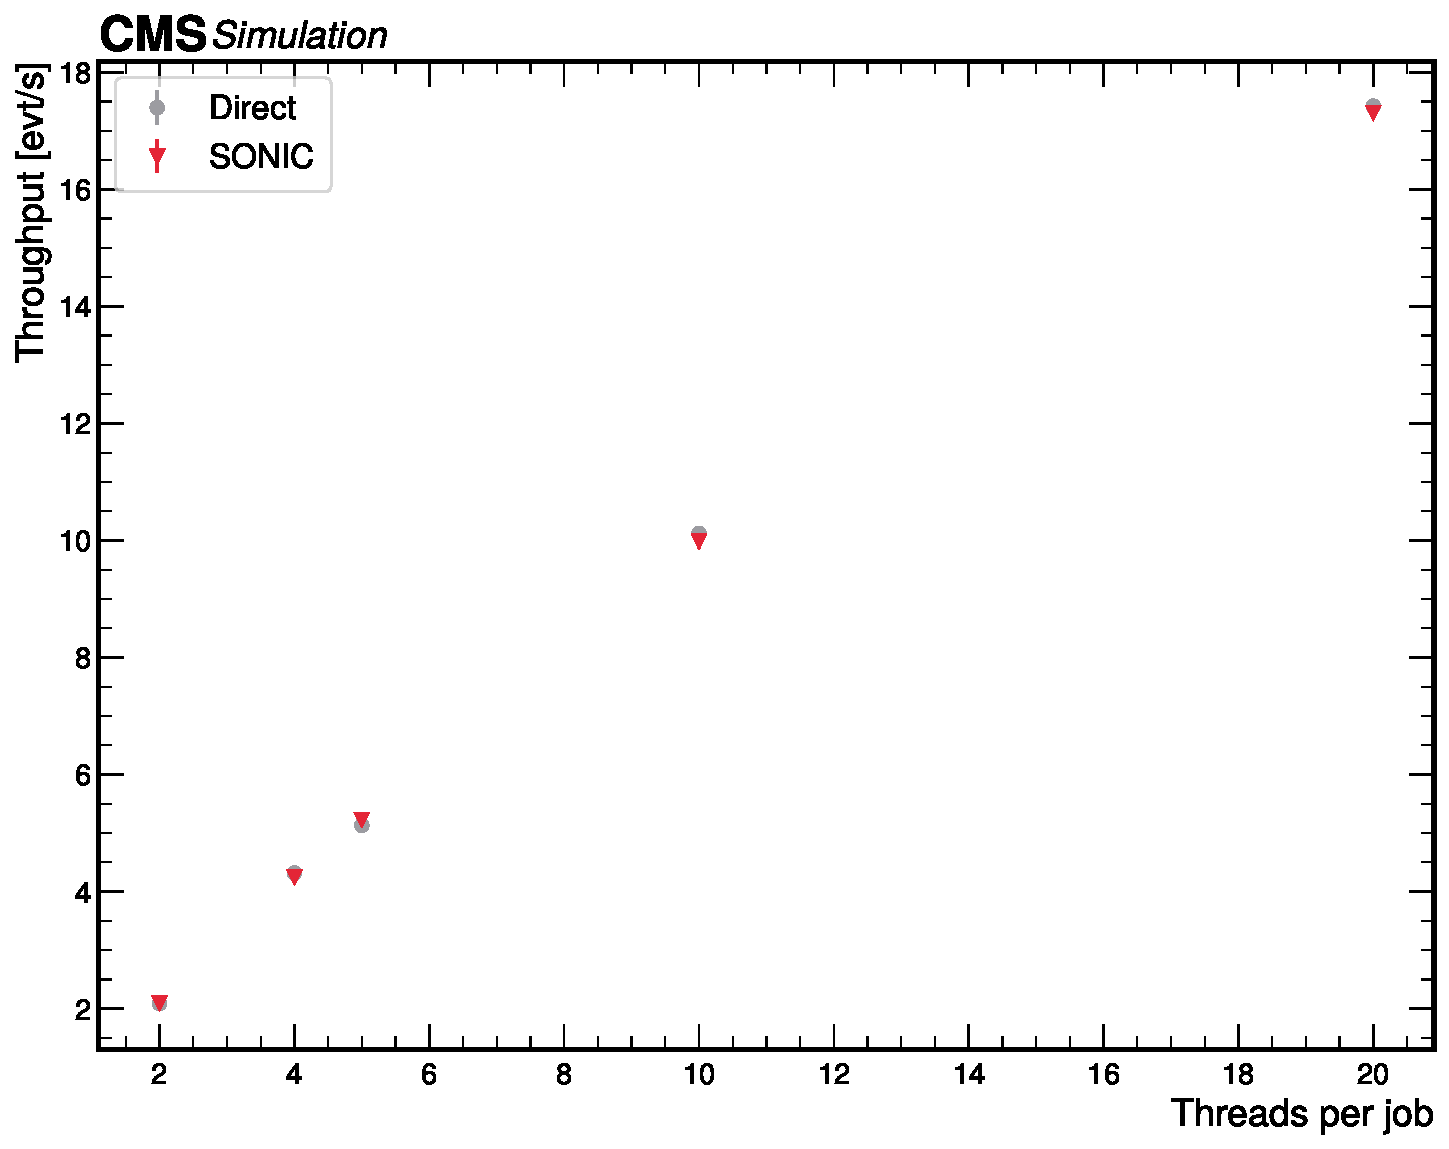
\includegraphics[width=0.48\textwidth]{plots/threads_vs_throughput.pdf}
    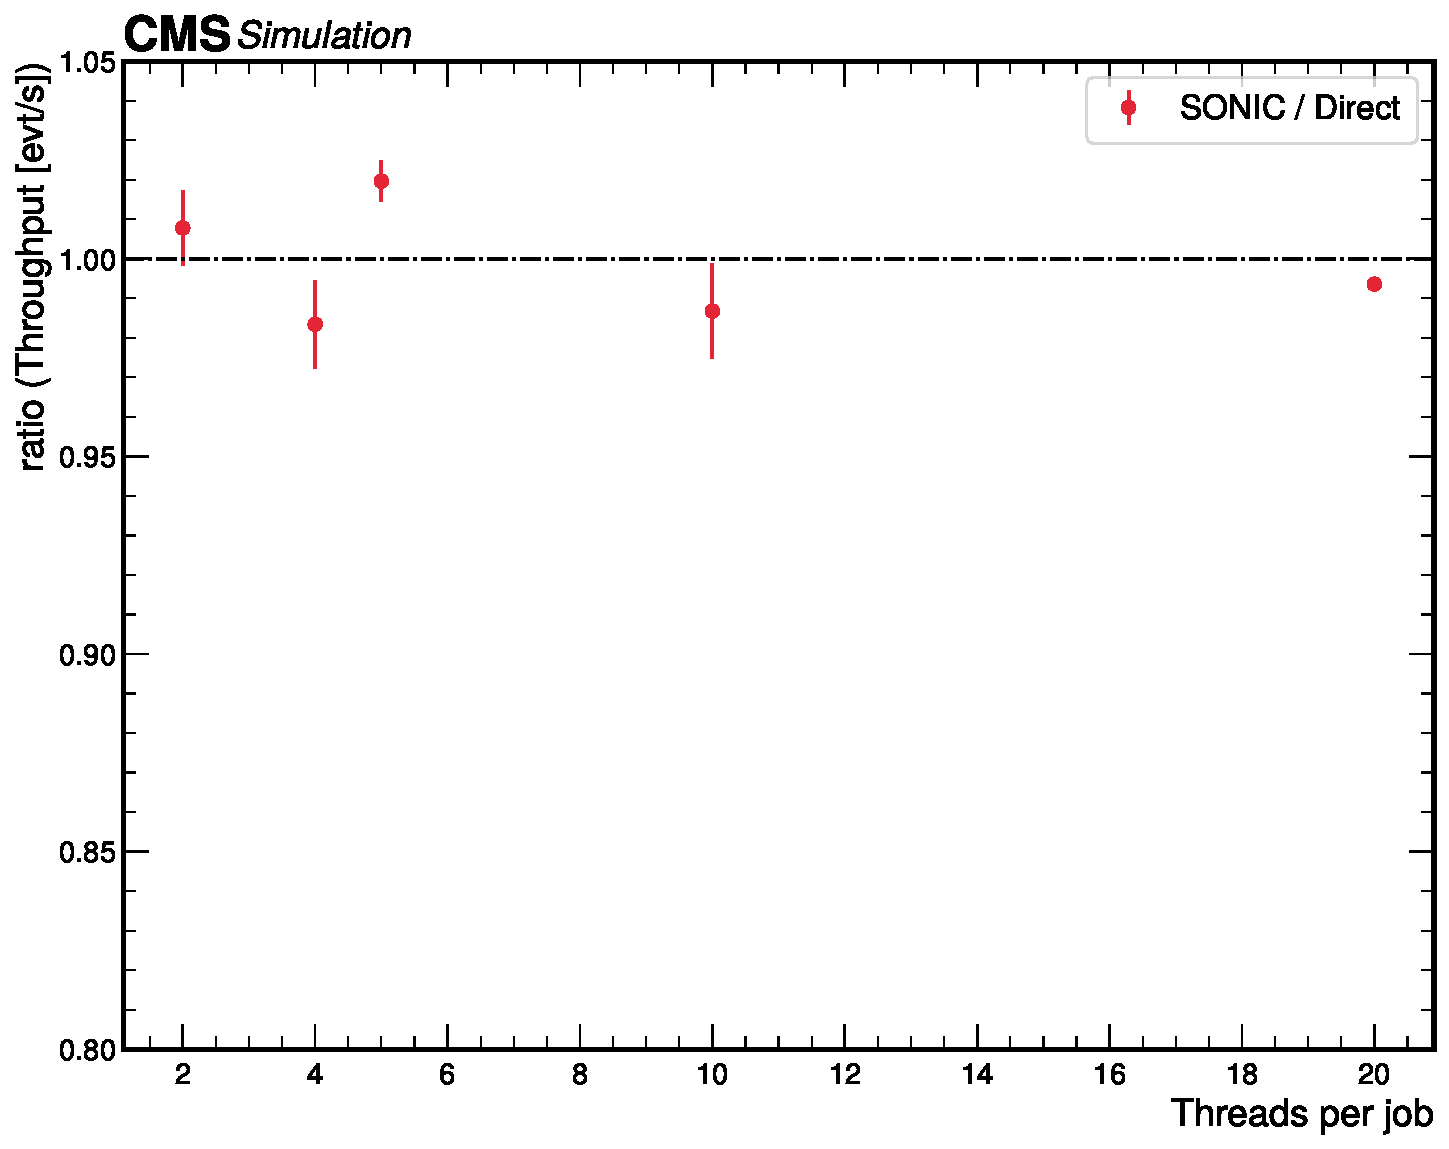
\includegraphics[width=0.48\textwidth]{plots/threads_vs_throughput__ratio.pdf}
    \caption{Throughput (left) and throughput ratios (right) of different configurations of the CPU saturation tests at Purdue Tier-2 Cluster.}
    \label{fig:throughput_cpu}
\end{figure}


\subsection{Studies with Graphcore IPUs}
\textcolor{red}{Detailed contents are still under discussion with GraphCore team.}

As discussed in Sections~\ref{sec:triton} and~\ref{sec:sonic_benefits}, NVIDIA Triton inference servers support custom backends to run with different coprocessors and different (ML) backends. Since the SONIC client code only depends on the Triton protocols, algorithms implemented in this way can easily be ported to different types of coprocessors. One of the Mini-AOD production tests was done together with the GraphCore IPU team, where they prepared a custom backend to support running ML inference with IPUs. The current supported ML frameworks include \TENSORFLOW and \PYTORCH, with \ONNX and \PYTORCHGEOMETRIC support in development. This allows us to run DeepMET and DeepTauID inference on IPUs. Without any modifications on the client side, we reconfigure the workflow configuration to point the clients to IPU servers on the Graphcloud cluster, and successfully run DeepMET and DeepTauID models via SONIC, while running the other parts of the Mini-AOD workflow on local CPUs.
